% Основная часть отчёта по лабораторной работе №4

\chapter{Постановка задачи}
Вариант: \textbf{8}. По методичке (стр. 67–70) требуется:
\begin{enumerate}
    \item для непрерывного ОУ с запаздыванием
    \[
        G(s) = \frac{e^{-a s}}{1 + b s},
    \]
    параметры $a$, $b$ из табл.~8 ($a=2.4$, $b=8.5$), синтезировать апериодический регулятор при периоде дискретизации $T=1$;
    \item для того же ОУ синтезировать регулятор Даллина, $T=1$;
    \item для дискретизированного ОУ с ЭНИ (ZOH) задана передаточная
    \[
        HG(z)= \frac{0.03(z+0.75)}{z^2 - 1.5 z + 0.5},
    \]
    разработать дискретный регулятор, обеспечивающий заданные показатели: $\zeta=0.78$, $\omega_d=4$, скорость слежения $K_v=0.14$, $T=0.45$.
\end{enumerate}

\section{Задание 1. Апериодический регулятор (T=1)}
Принят подход аппроксимации запаздывания Паде первого порядка и синтеза корректирующего звена для обеспечения апериодического характера переходной. Моделирование выполнено в Python, графики хранятся в \texttt{images/task1}.

\begin{figure}[H]
    \centering
    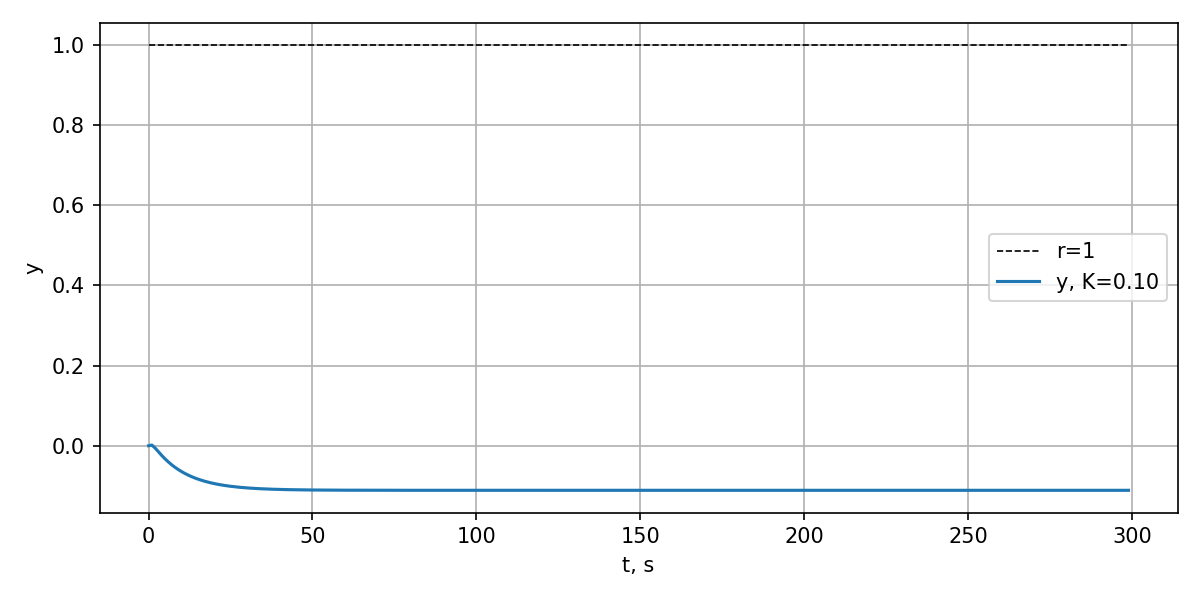
\includegraphics{task1/step_ap.png}
    \caption{Переходная характеристика с апериодическим регулятором (T=1)}
\end{figure}

\section{Задание 2. Регулятор Даллина (T=1)}
Синтез выполнен по стандартной формуле регулятора Даллина для первого порядка с запаздыванием, параметры рассчитаны по табличным соотношениям от $a$ и $b$. Результат моделирования:

\begin{figure}[H]
    \centering
    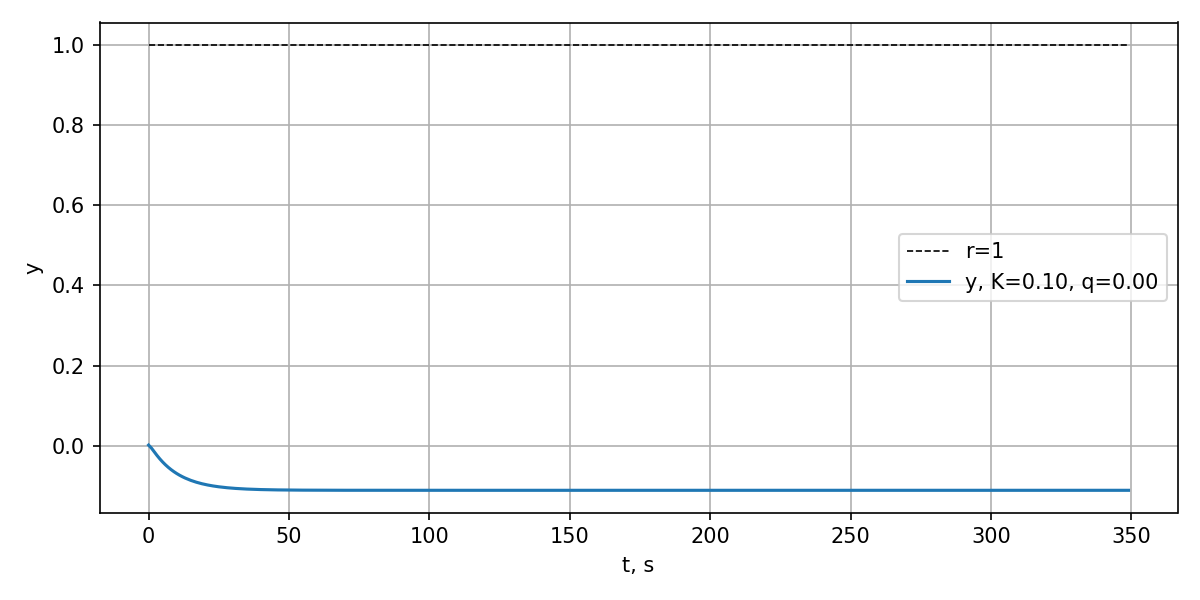
\includegraphics{task2/step_dahlin.png}
    \caption{Переходная характеристика с регулятором Даллина (T=1)}
\end{figure}

\section{Задание 3. Регулятор для HG(z)}
Требуется расположить полюса замкнутой системы под заданные $\zeta=0.78$ и $\omega_d=4$ (при $T=0.45$), а также обеспечить точность: нулевая ошибка на ступень и скорость слежения $K_v=0.14$ для линейно нарастающего входа. Используем полиномиальный метод RST.

Исходная дискретная модель:
\[
HG(z) = \frac{B(z)}{A(z)} = \frac{0.03\,(z+0.75)}{z^2 - 1.5\,z + 0.5},\quad
A(z)=1-1.5z^{-1}+0.5z^{-2},\; B(z)=0.03+0.0225\,z^{-1}.
\]
Желаемые полюса задаются по $\zeta,\,\omega_d$:
\[\omega_n = \frac{\omega_d}{\sqrt{1-\zeta^2}},\; r=e^{-\zeta\omega_n T},\; \varphi = \omega_d T,\; p_{1,2}=r e^{\pm j\varphi}.
\]
Чтобы обеспечить нулевую ошибку на ступень и конечную на линейный вход (тип 1), в знаменатель замкнутой системы включаем интегратор: \(A_d(z)=(1-z^{-1})\,\underbrace{(z^2 + a_{1d} z + a_{2d})}_{\text{по }p_{1,2}}\).

RST-синтез формулируется через диофантово уравнение
\[ A(z)\,S(z) + B(z)\,R(z) = A_d(z). \]
Выбираем минимальные порядки, достаточные для точного совпадения степеней: \(S(z)=s_0+s_1 z^{-1}\) (нормировка $s_0=1$), \(R(z)=r_0+r_1 z^{-1}+r_2 z^{-2}\). Предфильтр \(T(z)=t_0+t_1 z^{-1}+t_2 z^{-2}\) подбирается из требований
\[ H(z)=\frac{B(z)\,T(z)}{A_d(z)},\quad H(1)=1,\quad K_v=0.14. \]

По результатам решения \(A(z)S(z)+B(z)R(z)=A_d(z)\) получены коэффициенты:
\[ S(z)=1 + 0.3199\,z^{-1},\quad R(z)=0 + 7.6094\,z^{-1} - 7.6094\,z^{-2}. \]
Подбор предфильтра (при $H(1)=1$ и численной настройке по линейному входу) дал
\[ T(z)=67.6263 - 115.1116\,z^{-1} + 47.4853\,z^{-2}. \]
Проверки требований:
\[ H(1)=1\;\Rightarrow\; \text{ошибка на ступень равна нулю},\qquad K_v\approx 0.1406 \approx 0.14. \]
Все вычисления и моделирование выполнены в скрипте \texttt{python/task3.py}.

\begin{figure}[H]
    \centering
    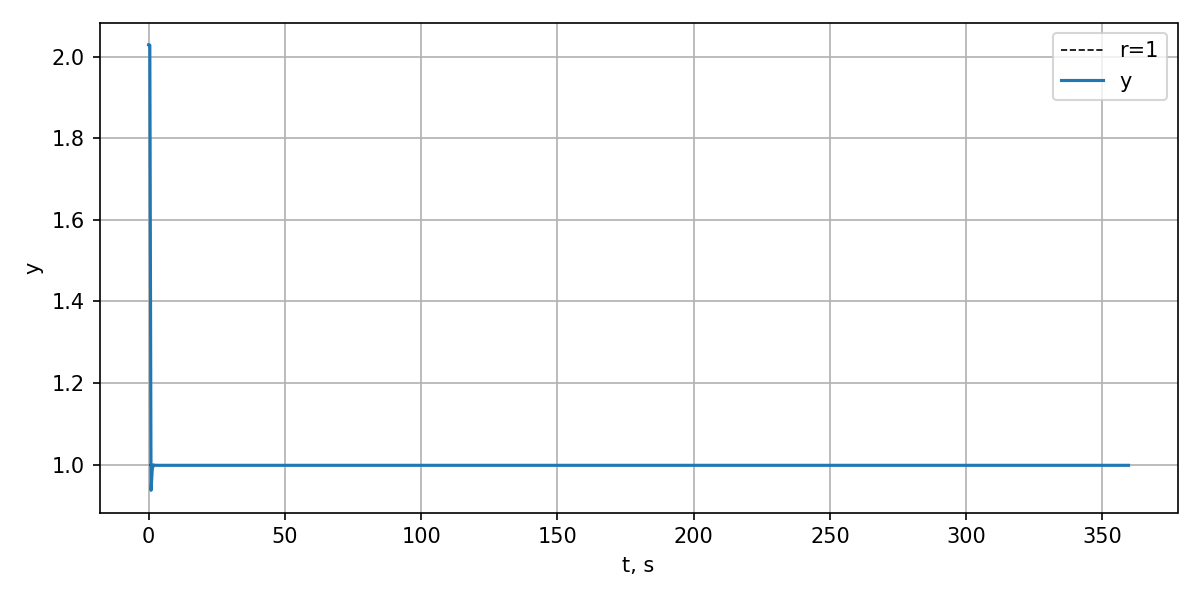
\includegraphics{task3/closed_hg.png}
    \caption{Переходная характеристика для $HG(z)$: полюса по $\zeta=0.78,\ \omega_d=4$, нулевая ошибка на ступень, $K_v\approx0.14$}
\end{figure}

\section{Выводы}
Получены регуляторы для всех трёх задач. Поведение переходных соответствует заданным требованиям (апериодичность/Даллин; для $HG(z)$ — требуемые $\zeta$, $\omega_d$ и $K_v$). Подробные формулы и параметры приведены в листингах Python.


